%% This document gives an example on how to use the ntnumasterthesis
%% LaTeX document class.

%% Use short name MACS, MIS, CIMET, MTDMT, MIXD or MIS  
%% Language english or norsk
%% b5paper with oneside or twoside, you can set A4 if you want but you submit in b5

%% If you want print with the heading material on a4 paper you can use this format
%% \documentclass[MACS,english,a4paper,oneside,12pt]{ntnuthesis/ntnuthesis}

%% with the change to using DAIM we have a new option.
\documentclass[MACS,english,DAIM]{ntnuthesis/ntnuthesis}

\usepackage[T1]{fontenc}
\usepackage[utf8]{inputenc}     % For utf8 encoded .tex files allows norwegian characters in the files. This can be dangerous if you change to a differnt editor.
%\usepackage[pdftex]{graphicx, hyperref}   % For cross references in pdf
\usepackage{graphicx}
\usepackage{hyperref}   % For cross references in pdf


\usepackage{color}              % For colouring text 
\hypersetup{colorlinks=true,     
		linkcolor=blue,          % color of internal links (change box color with linkbordercolor)
    citecolor=blue,        % color of links to bibliography
    filecolor=blue,      % color of file links
    urlcolor=blue           % color of external links
		}
\usepackage{csvsimple}  % for simple table reading and display
\usepackage{url}

% Set to true ONLY if using Harvard citation style
\newboolean{HarvardCitations}
\setboolean{HarvardCitations}{false} % false for computer science, true for interaction design and harvard style


\ifthenelse{\boolean{HarvardCitations}}{%
	\usepackage{natbib} % for Harvard names as citations.
}{%
	\usepackage[numbers]{natbib} % for Vancover numbers in bibliography
}



\begin{document}

% for students submitting in the DAIM system this information will not be used.
% their is an option for DAIM submission which removes this information and checks it is B5.
% The nonDAIM option will use this material.

\setthesistitle{Example Masters Thesis. With a long title to test the wrapping of the box}
\setthesisauthor{Simon McCallum}
\setthesissupervisor{Assoc. Prof. Nils Kalstad Svendsen}
\setthesissupervisorA{Prof. Jon Yngve Hardeberg}  % if you have a second supervisor add it like this


\nmtkeywords{Thesis, Latex, Template, IMT}
%\nmtdesc{This is the short description of a masters thesis}


\setthesisdate{31-05-2017}
\setthesisyear{2017}



%for CIMET theses you need to see all of these as well

%\setthesiscampus{Gj\o{}vik}
%\setthesisHostInstitution{\NTNU}
%\setthesisHostInstitution{University of Eastern Finland}
%\setthesisHostInstitution{Universit\'e Jean Monnet Saint-Etienne}

%\setthesisjuryA{} %jury names
%\setthesisjuryB{} %jury names
%\setthesisjuryC{} %jury names
%\setthesisjuryD{} %jury names


 % this is the file which contains all the details about your thesis
\makefrontpages % make the frontpages
%this is the intro to the thesis
%\thesistitlepage % make the ordinary titlepage
\hypersetup{pageanchor=false}
%\include{summary}

\addcontentsline{toc}{chapter}{Preface}
\chapter*{Preface}
Here, you give a brief introduction to your work. What it is (e.g., a Master's thesis in AIMT at NTNU, when it was carried out (e.g., during the autumn semester of 2021). If the project has been carried out with a company, you should mention this and also describe the cooperation with the company. You may also describe how the idea to the project was brought up.

You should also specify the assumed background of the readers of this report (who are you writing for).\\[2cm]

%\begin{center}
%\thesiscampus, 
\thesisdate \\[1pc]
\\[1pc]
%\thesisauthor
%\end{center}

\addcontentsline{toc}{chapter}{Acknowledgment}
\chapter*{Acknowledgment}
I would like to thank the following persons for their great help during \ldots

If the project has been carried out in cooperation with an external partner (e.g., a company), you should acknowledge the contribution and give thanks to the involved persons.

You should also acknowledge the contributions made by your supervisor(s).

\begin{flushright}
O.N.\\[1pc]
(Your initials)
\end{flushright}

\addcontentsline{toc}{chapter}{Abstract}
\chapter*{Abstract}

This is a summary of the thesis including the conclusion of what was discovered.

\hypersetup{pageanchor=false}



\tableofcontents

\hypersetup{pageanchor=true}

% Comment with a percent to remove figures or tables:
\listoffigures
\listoftables


\chapter{Introduction}
\label{chap:introduction}

 These detailed
typographical rules have been implemented in the
\texttt{ntnuthesis} \LaTeX\ document class.

The purpose of this document is to provide an example and description
on how this class file can be used.

This was then extended to include bachelor project by Simon McCallum.
The package has changed names and version number it is now called
\texttt{ntnuthesis}
v\ntnuthesisversion\ as of \ntnuthesisdate. % includes latex files from the same directory
\chapter{Packages}
\label{chap:packages}

The \texttt{ntnuthesis} is built upon the standard \LaTeX\
\texttt{report} class. All commands from the \texttt{report} class can
be used, with the two exceptions of \verb+\subsubsection+ and
\verb+\paragraph+. This is because there should only be three
levels of headings according to the guidelines. 
It has been placed in a folder called \texttt{ntnuthesis} so that it does not
clutter your work.  You should not change anything in \texttt{ntnuthesis}

\section{Packages Used by ntnuthesis}
\label{sec:packages}

In addition to the \texttt{report} document class,
\texttt{ntnuthesis} makes direct use of the following packages
that must hence be present:
\begin{description}
	\item[geometry:] used for setting the sizes of the margins and
  	headers.
	\item[fontenc:] used with option \texttt{T1} for forcing the Cork font
  	encoding (necessary for the Charter font).
	\item[charter:] load Charter as the default font.
	\item[euler:] load the Euler math fonts.
	\item[bable:] for language handling.
\end{description}

\section{Other Relevant Packages}
\label{sec:otherpackages}

The author of a thesis might want to use a bunch of different packages
to those described in Section~\ref{sec:packages} in order to have all features needed for their document. 
In particular, it is advised to use the following:
\begin{description}
	\item[inputenc:] to allow \LaTeX\ to use more than 7-bit ASCII for its
	  input. Most often, the option \texttt{latin1} will do.
	\item[babel:] to load language specific strings. Reasonable options
	  include \texttt{british}, \texttt{american}, \texttt{norsk} and
	  \texttt{nynorsk}.
	\item[graphicx:] to include graphics.
	\item[hyperref:] this is a very nice package that makes cross links in
	  pdf documents. Use with option \texttt{dvips} or \texttt{pdftex}
	  in accordance with the driver that you use. Unfortunately, hyperref
	  is not completely bugfree\dots
\end{description}

We have web pages as well~\cite{NTNU:Website}, and now games like Halo~\cite{Halo}. % could be called Methodology or methods or anyfile name 
\chapter{Structural Elements}
\label{chap:structural}

The title of the thesis should be set using the \verb+\thesistitle+
command, and the date of the thesis should be set using the
\verb+\thesisdate+ command. This makes the title and date appear in
the running header, like in this document.

\section{Page Layout}

The geometry of the page has been set using the \verb+\geometry+
command.

\section{Fonts}

Due to limited \LaTeX\ support for the Georgia font, Charter has been
chosen instead. For mathematical formula, the Euler fonts are used,
since they blend more nicely with the Charter than the standard
\LaTeX\ fonts: 
\begin{equation} \label{eq:1}
    f(x) = \int_0^x g(\tau)\,d\tau
\end{equation}



For inline math you can use $\backslash{}($ and $\backslash{})$ for example \( f(x)= \frac{x^2}{1+x^2} \).  
This also allows you to use $\slash$ and $\backslash$. You need to include the \{\} when you want the special
character to have other letters immediately after it.

\section{Sectioning Commands}

The standard \LaTeX\ sectioning commands are used for both numbered
and unnumbered sections. The top level is given by the \verb+\chapter+
command. This starts a new right page. The two lower levels are
obtained using the \verb+\section+ and \verb+\subsection+ commands.
The standard \LaTeX\ \verb+\subsubsection+ and \verb+\paragraph+
commands have been disabled since their use is not encouraged by the
thesis guidelines. When you use these they will not be given numbers.  
They still appear in the document with highlighting but not in the 
table of contents.

\subsection{The subsection}

This is an example of a subsection.

\subsubsection{The subsubsection}

This is an example of a subsubsection.

\paragraph{The paragraph}

This is an example of a paragraph with a heading.

\section{Floats (Figures and Tables)}
\label{sec:floats}

Figures are placed in the \texttt{figure} environment. An example is
shown in Figure~\ref{fig:example}. %notice the ~ in between figure and the \ref. it stops latex from splitting the number and word over a line.
Tables are placed in the \texttt{table} environment. An example is given in
Table~\ref{tab:example}. Figures and tables float freely around in the
document in accordance with standard \LaTeX\ behavior.

\begin{figure}[tbp]  %t top, b bottom, p page | you can also use h to try to get the figure to appear at the current location
  \centering
  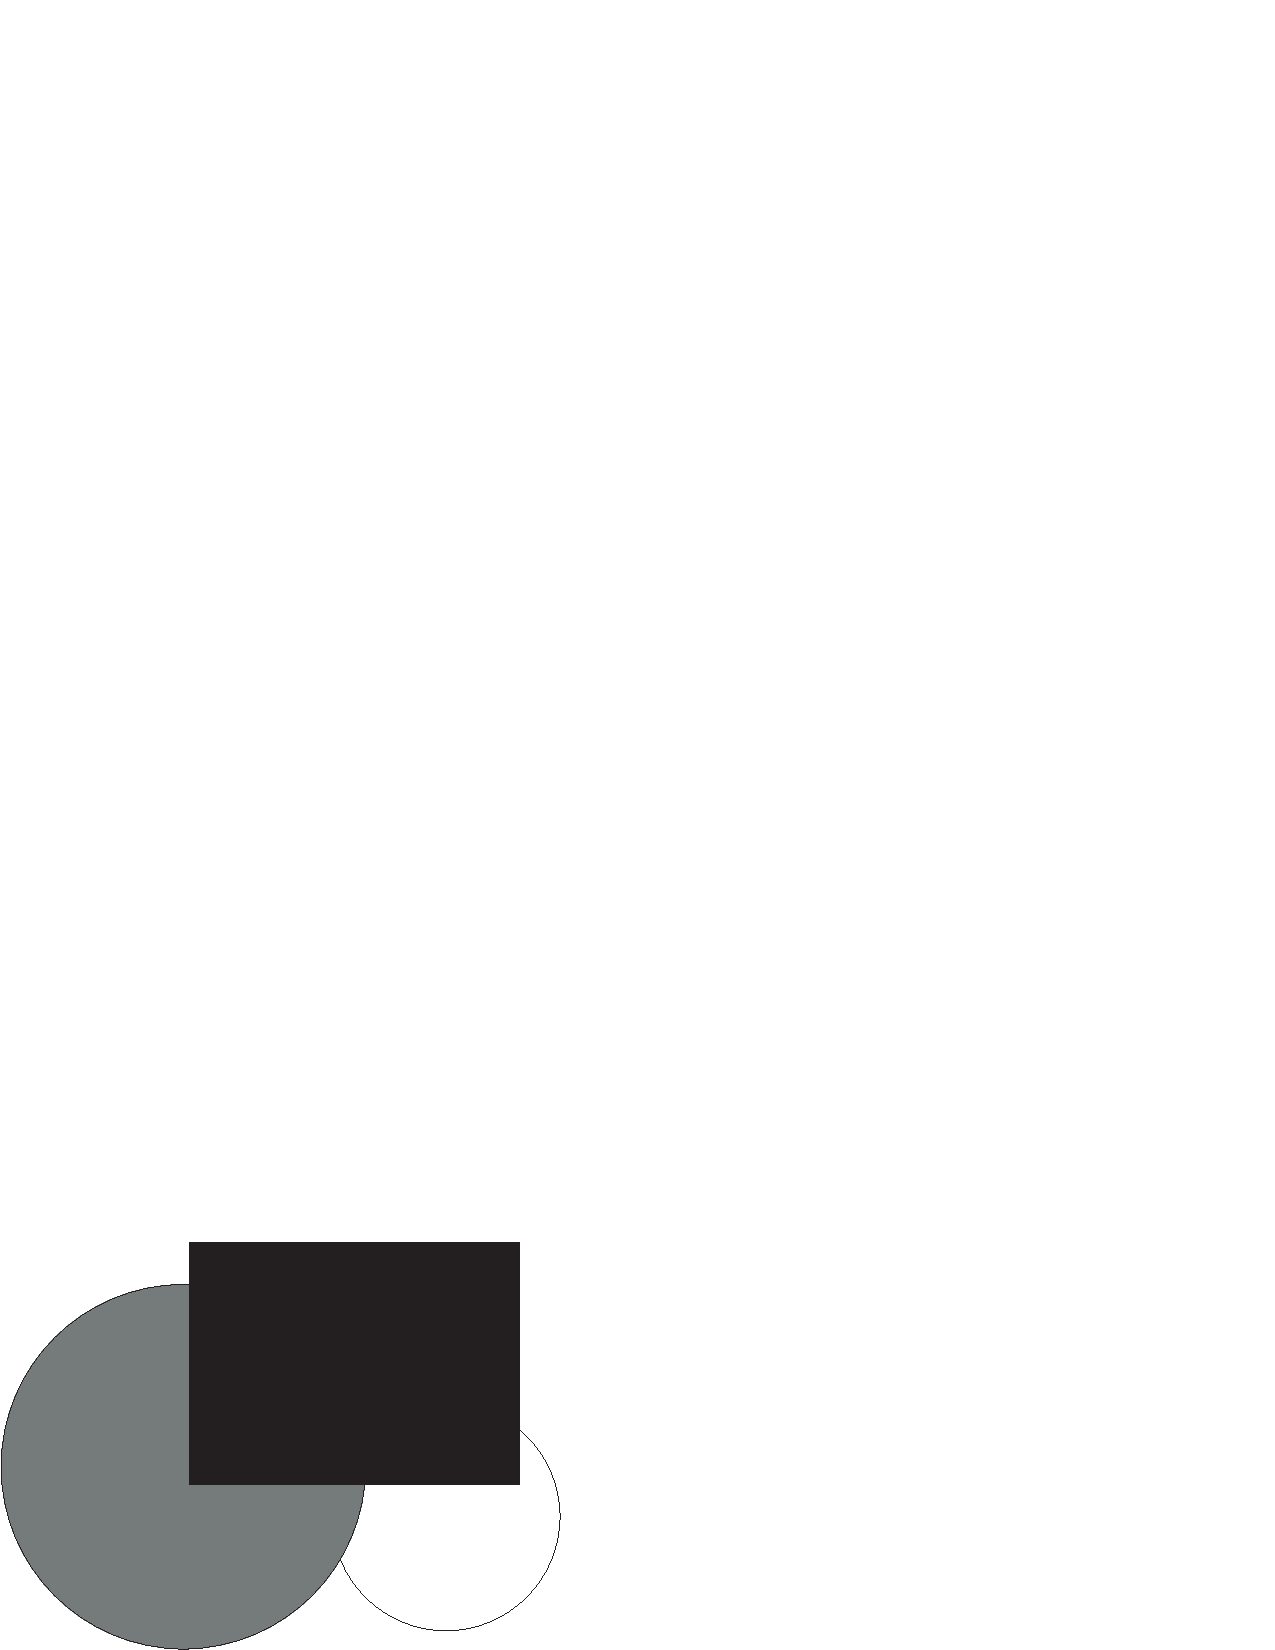
\includegraphics[width=.5\textwidth]{figures/example_fig}
  \caption[An example figure.]{An example figure. If the caption is
    shorter than one line, it is centered. If it goes over more than
    one line, it is left and right justified. Furthermore, it is
    suggested that an alternative short caption is given in order to
    produce a good list of figures.}
  \label{fig:example}
\end{figure}

\begin{table}[tbp]
  \centering
  \begin{tabular}{c|c}
    Age  & IQ  \\ 
    \hline
    10   & 100 \\
    20   & 100 \\
    30   & 150 \\
    40   & 100 \\
    50   & 100
  \end{tabular}
  \caption{An example table.}
  \label{tab:example}
\end{table}

The captions are placed \emph{below} both for the figures and the
tables. The caption is set in 9pt. If the caption is shorter than one
line, it is centered.

\section{Quotes}
\label{sec:Quotes} % this allows you to refer to this section number using \ref{sec:Quotes}

Quotes are inserted using the standard \LaTeX\ \texttt{quote}
environment. The environment has been changed so that a 9pt font is
used:

\begin{quote}
  ``And I looked, and, behold, a whirlwind came out of the north, a
  great cloud, and a fire infolding itself, and a brightness was about
  it, and out of the midst thereof as the colour of amber, out of the
  midst of the fire. Also out of the midst thereof came the likeness
  of four living creatures.''
\end{quote}

\section{Lists}
\label{sec:lists}

Point lists and enumerated lists are made by using the standard
\texttt{itemize} and \texttt{enumerate} environments, respectively.
The spacing is going to be changed in accordance with the specification. For
\texttt{itemize}, the results look like this:
\begin{itemize}
	\item First item.
	\item Second item. Here I will put some long text, just to illustrate.
	  Here I will put some long text, just to illustrate. Here I will put
	  some long text, just to illustrate. Here I will put some long text,
	  just to illustrate.
	\item Third item also has subitems:
	  \begin{itemize}
		  \item First subitem.
		  \item Second subitem.
		  \item Third subitem.
	  \end{itemize}
\end{itemize}
and for \texttt{enumerate} like this:
\begin{enumerate}
	\item First item.
	\item Second item. Here I will put some long text, just to illustrate.
	  Here I will put some long text, just to illustrate. Here I will put
	  some long text, just to illustrate. Here I will put some long text,
	  just to illustrate.
	\item Third item also has subitems:
	  \begin{enumerate}
		  \item First subitem.
		  \item Second subitem.
		  \item Third subitem.
	  \end{enumerate}
\end{enumerate}

You may also want to use descriptive lists
\begin{description}
	\item[First] the first item.
	\item[Second] the second item. Here I will put some long text, just to illustrate.
	  Here I will put some long text, just to illustrate. Here I will put
	  some long text, just to illustrate. Here I will put some long text,
	  just to illustrate.
	\item [What now] the third item also has subitems:
	  \begin{enumerate}
		  \item First subitem.
		  \item Second subitem.
		  \item Third subitem.
	  \end{enumerate}
\end{description}


\section{Bibliographic References}

There are two distinct styles of referencing which can be used within the Masters thesis, Vancouver for Computer Science and Harvard for Interaction Design.

In Computer Science we generally use the Vancouver style with numbered references.  
I have added a boolean option \verb| \setboolean{HarvardCitations}{false} |  Havard style if false for computer science and true for interaction design.
 
In the Vancover style you should cite articles~\cite{Askvall1985}, books~\cite{Card1983},
anthologies~\cite{Lancaster1985} and web publications~\cite{Meldon1997}
like this. For all citations note that in the text there is the tilde \~ character.  
That is a non-breaking space which forces the number to stay with the text rather than move to the next line.
There is always an issue referencing web pages. Currently
we suggest that you use the NTNU Website~\cite{NTNU:Website}.


For Harvard style referencing, you use the \texttt{citep} and \texttt{citet} style of citation. 
These give parentheses around the citation or the name of the author as text with the year in parentheses.  
If you want the citation to be read in a sentence then you use  \texttt{citet}. 
If you want it to be just parenthetical to the sentence at the end, then use \texttt{citep}.




 % could be results

\chapter{Conclusion}
\label{chap:conclusion}

% in rw datasets you deal with what you have. For instance, labels in parent categories should be used
% in the standard dt they take images, then desing categories and then manually or semimanually label them

TODO: While which network configuration to use should be considered in each particular case, the study gives some insights on how different decisions can influence both training performance and final system classification precision. Two different network architectures were tested The choice of the solver method can influence 
% Dataset splitting can be a challenge for multi-label classification case. Random sampling approach used in the main experiments of the study showed the best results in terms of the closest average ratio to the desired one. %The limitation on minimal number of images in one category can depend on how tightly connected are categories in the dataset and amout of images in them.  % not onlu real-world

The NTB dataset analysis together with the tree transformation performed revealed possible challenges and issues of building multi-label classification system based on real-world datasets:
\begin{itemize}
    \item Currently, modern neural networks do not incorporate hierarchical structure of the categories tree, therefore it has to be transformed to a flat structure. Depending on a specific dataset, different approaches can be used to perform this transformation. Characteristics of the dataset that should be considered include: if both parent and child categories are used to label images, if the relationship type between categories is consistent across the tree, and if the manual labeling rules are consistent. Depending on the dataset this process can be automatized to a certain level.
    \item There can be contextual, combined, too abstract, and ambiguous categories. Such categories should be explicitly separated from other ones before the training process in order to acheive better system performance. % more categoires -> less weights/neurons can be used for others
    %\item categories with different purpose?
    \item One of the main challenges is to deal with contextual images, which can be classified only with additional information. While manual separation of such images could give the best outcome, the study suggest approach that uses known connections between categories in order to filter out some part of such images automatically.
    \item Not consistent understanding and use of particular category between different manual labelers can result in reduced classification performance. However, results from the study suggest that in some cases it is still possible for a system to generalize on the category. This system can be further used to improve consistency in the initial dataset. % sign of triumph
    
    % \item duplicates
\end{itemize}

Results from the experiments show a big potential of fine-tuning pretrained convolutional neural networks in solving the problem of multi-label image classification on a real-world dataset. The actual level of classification for a particular dataset performance will depend on its quality and size. However, the results chapter can give indication of which classification system performance level can be achieved when training on a dataset similar to the one used in the research.
% However, it is expected that correlations and insights will likely to be applicabe to other real-world datasets as well.
Further investigation of the trained networks shows that due to existing errors in the original dataset, the end classification system performance can be even better than suggested by the results.

Results suggest that improvement in the network architecture do not necessarily improve end classification performance. However, results also indicate that different neural networks can perform better in different conditions. For example, more modern GoogleNet architecture compared to older CaffeNet showed better results for categories with larger sample size, but had opposite effect on the categories with small number of pictures.

% The manual work on the category tree is most likely required, but not necessarily on the image level. Results suggest that it is possible to further improve system performance by improving the dataset using available connections between categories (removing portrait and press-conference pics from sports categories) .. The next level would be to train network, use it to improve dataset and retrain it on it again.

% An additional discovery This fact also implies that small imperfections of the dataset do not influence the end performance on a big scale. %But in depends on the size of sample.


The main limitation of study is that all experiments were performed on the single available dataset, therefore the generalizability of results and insights is in question. Results are considered likely to be more generalizable to datasets similar to the one used in the study. Experiments were designed to maximize reproducablility and internal validity. However, further studies should be done to validate obtained results.


\ifthenelse{\boolean{HarvardCitations}}{%
	\bibliographystyle{agsm} % used for Harvard style references. Names - Humanities & Interaction Design
}{%
	\bibliographystyle{ntnuthesis/ntnuthesis} %used for Vancover style references. Numbers - Computer Science & Physics
}

\bibliography{MastersExample}

\appendix
\chapter{Signed contract with NTB}
\label{app:contract}
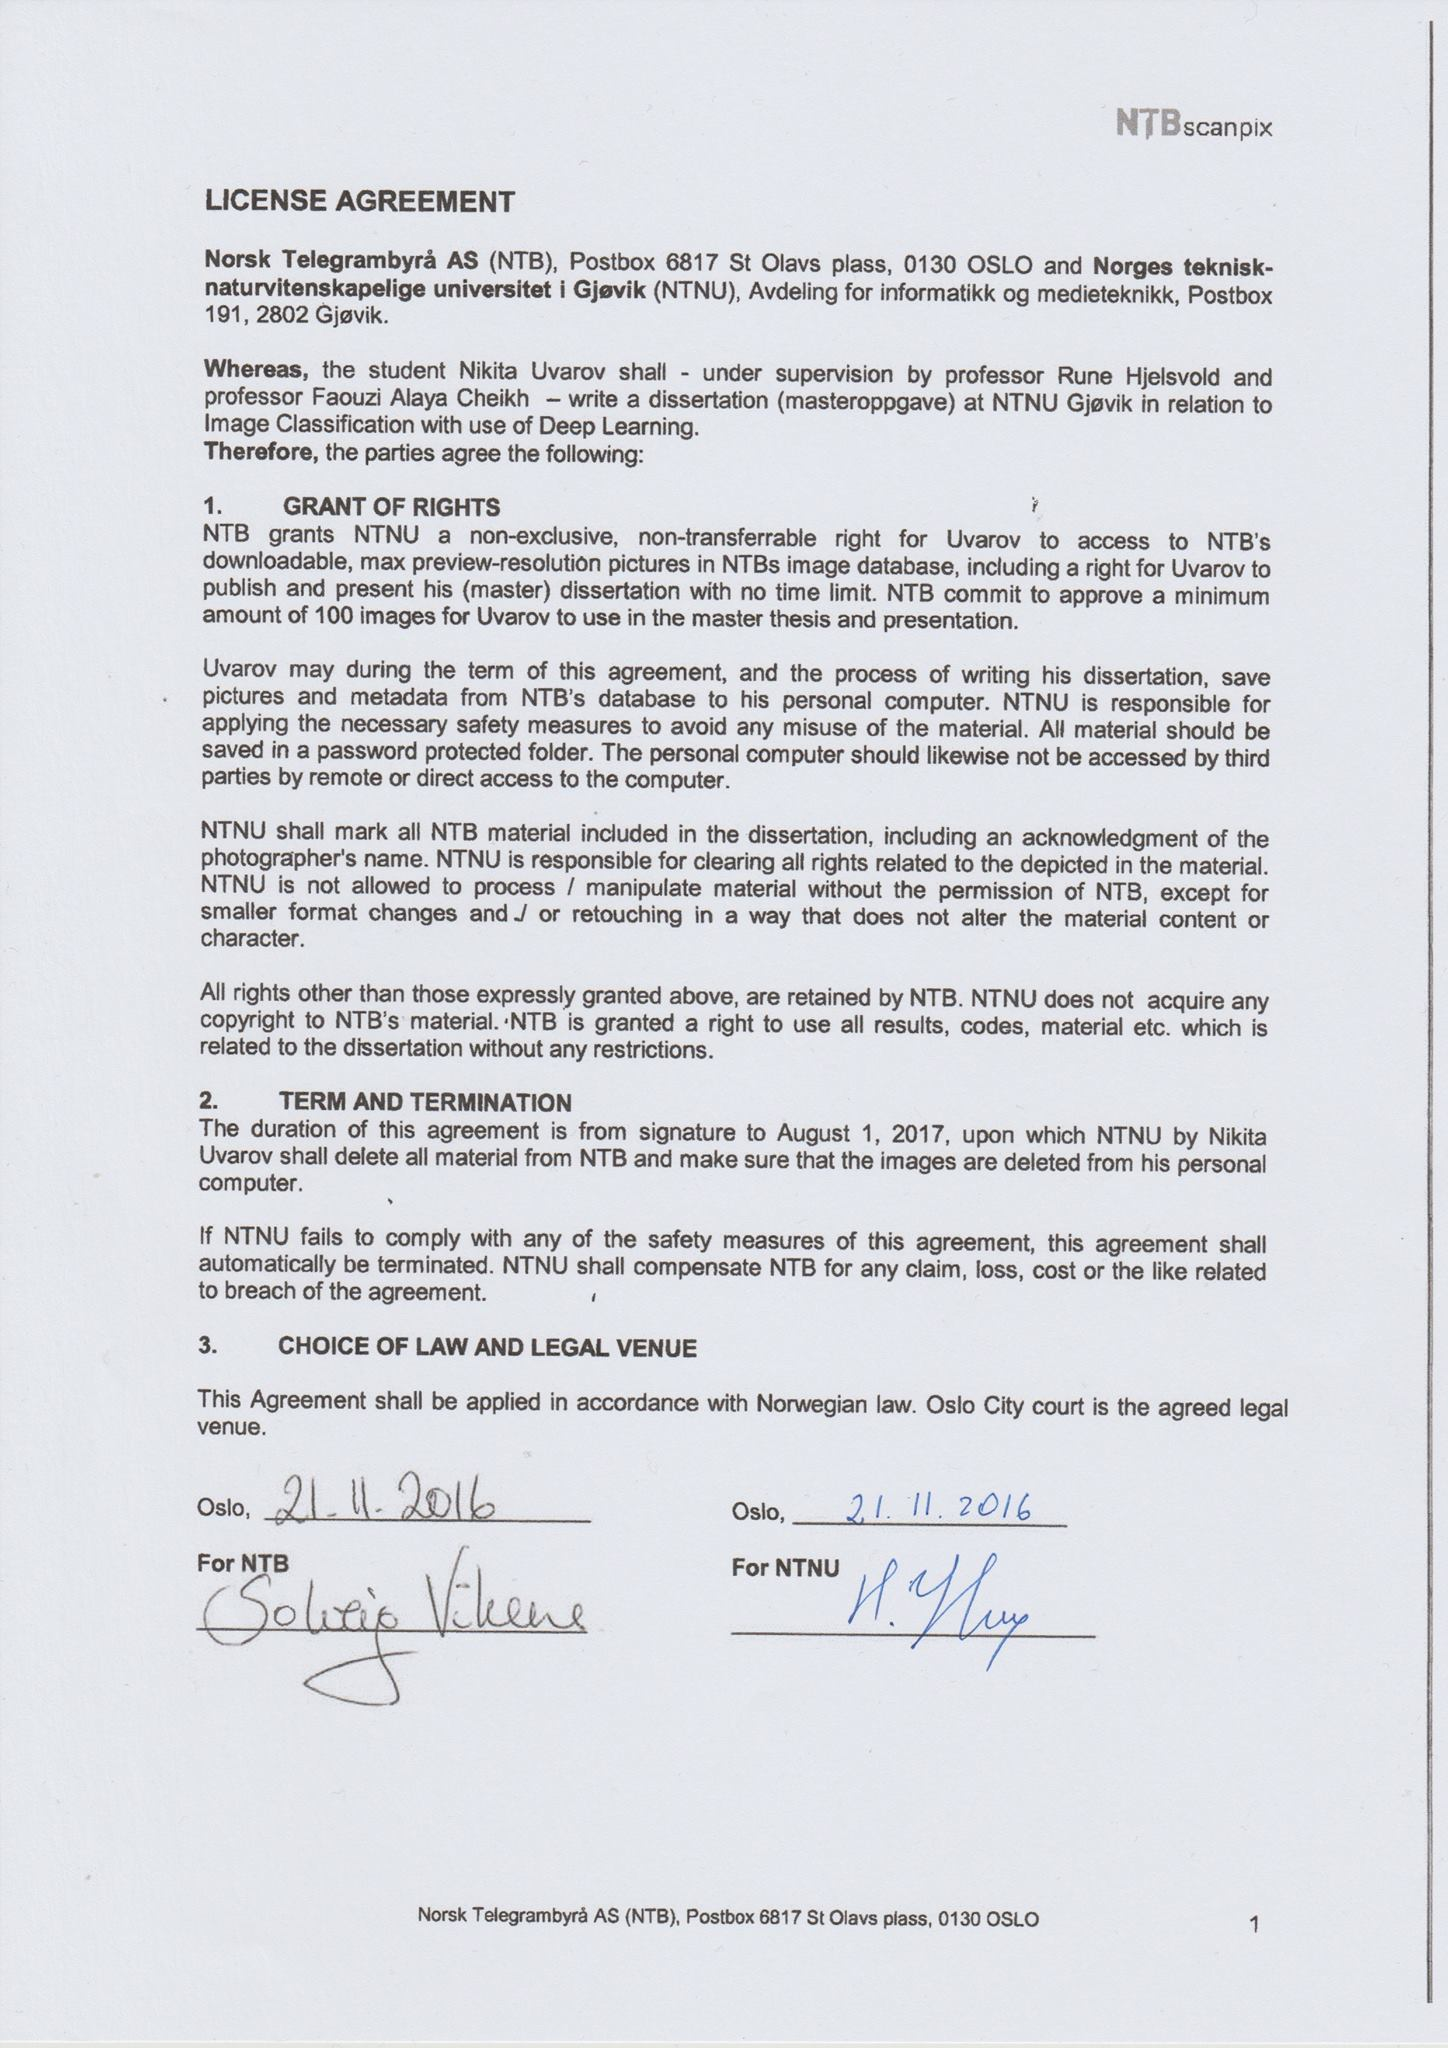
\includegraphics[width=0.9\textwidth]{contract}

\end{document}
